\documentclass[a4paper,10pt]{exam}

\usepackage[utf8]{inputenc}
\usepackage[cyr]{aeguill}
\usepackage[francais]{babel}
\usepackage{fullpage}
\usepackage{amsmath}
\usepackage{array}
\usepackage{tikz}
\input kvmacros
\usetikzlibrary{arrows,shapes,trees,patterns,fit,backgrounds,%
decorations.pathreplacing,chains,calc,decorations.pathmorphing,matrix,circuits.logic.CDH}

\ifthenelse{\equal{\detokenize{correction}}{\jobname}}
{\printanswers}
{\noprintanswers}

\title{Architecture des ordinateurs - TD 07}

\author{}
\date{}

\begin{document}
\maketitle

\section{Circuits additioneurs (retour)}
\begin{enumerate}
\item Un demi additionneur est composé de:
  \begin{itemize}
  \item deux entrées: les bits $a$ et $b$
  \item deux sorties: $s$ la somme des deux bits et $r$ l'éventuelle retenue.
  \end{itemize}
  Donner les expressions booléennes de $s$ et $r$ en fonction de $a$ et $b$.
\begin{solution}
  $s = a \oplus b$ et $r = ab$.
\end{solution}
\item Proposer un circuit pour le demi additionneur.
\begin{solution}
\begin{tikzpicture}[circuit logic CDH,
tiny circuit symbols,
every circuit symbol/.style={
fill=white,draw}]
\matrix[column sep=0.7cm, row sep=0.7cm]
{
\node (A) {a};  & \node [xor gate] (x) {};& \node (S) {s};  \\
\node (B) {b};  & \node [and gate] (a) {};& \node (R) {r};\\
};
\draw (A.east) -- ++(right:3mm) |- (x.input 1);
\draw (B.east) -- ++(right:6mm) |- (x.input 2);
\draw (A.east) -- ++(right:3mm) |- (a.input 1);
\draw (B.east) -- ++(right:6mm) |- (a.input 2);

\draw (x.output) -- ++(right:3mm) |- (S.west);
\draw (a.output) -- ++(right:3mm) |- (R.west);
\end{tikzpicture}
\end{solution}
\item Un additionneur complet est composé de:
  \begin{itemize}
    \item trois entrées: les bits $a$ et $b$ et $r_0$ la retenue
      propagé par l'additionneur précédent.
    \item deux sorties: $s = a + b + r_0 [2]$ et $r_1$ l'éventuelle retenue lors
      du calcul de $s$.
  \end{itemize}
  Construire un circuit pour l'additionneur complet. Pour cela utiliser
  deux demi-additionneur ainsi qu'une porte OU.

\begin{solution}
\begin{tikzpicture}[circuit logic CDH,
tiny circuit symbols,
every circuit symbol/.style={
fill=white,draw}]
\matrix[column sep=0.7cm, row sep=0.7cm]
{
\node (A) {a};  &                                                    & &&\\
                & \node[draw] (ha1) {$\frac{1}{2}+$}; & \node[draw] (ha2) {$\frac{1}{2}+$};& \node (outs) {s};&\\
\node (B) {b};  & \node (R)[yshift=3mm] {$r0$};                   &                                    &\node (o) [or gate] {}; & \node (outr) {r};\\
};
\draw (A.east) -- ++(right:3mm) |- ([yshift=1mm]ha1.west) ;
\draw (B.east) -- ++(right:6mm) |- ([yshift=-1mm]ha1.west);
\draw ([yshift=1mm]ha1.east) -- ++(right:3mm) |- ([yshift=1mm]ha2.west);
\draw (R.east) -- ++(right:6mm) |- ([yshift=-1mm]ha2.west);

\draw ([yshift=-1mm]ha1.east) -- ++(right:3mm) |- (o.input 2);
\draw ([yshift=-1mm]ha2.east) -- ++(right:3mm) |- (o.input 1);


\draw (o.output) -- (outr);
\draw (ha2.east) -- (outs);
\end{tikzpicture}
\end{solution}


\item Additionneur 4 bits. Un additionneur 4 bits possède 8 signaux en entrée et
  5 signaux en sortie:
  \begin{itemize}
    \item entrées: $A=a_3a_2a_1a_0$ et $B=b_3b_2b_1b_0$ deux nombres codés sur
      4 bits chacun.
    \item sorties: $C=c_3c_2c_1c_0$ et $r$. C est la somme de $A$ et $B$ et $r$
      l'éventuelle retenue.
  \end{itemize}
  En utilisant les circuits des questions précédentes proposer un circuit pour
  l'additionneur 4 bits.

\begin{solution}
    On met en série: demi-additionneur et trois additioneurs complets.
    La retenue se propage d'une additionneur au suivant.

    Attention le temps de calcul est limité par la propagagtion de la retenue. Pour des mots grande taille (16 bits), il vaut
    mieux utiliser des additionneurs plus complexes comme le Carry Look Ahead (CLA) addder.
\end{solution}

\item Soit deux nombres positifs: $A=a_3a_2a_1a_0$ et $B=b_3b_2b_1b_0$, implémenter
  le circuit de la fonction $C(A,B) = A < B$ \textbf{en utilisant un circuit
    additionneur}.
  \begin{solution}
    On se sert d'un additionneur 5 bits.
    On remarque que $A < B \equiv A - B < 0$.
    On peut obtenir $-B$ en CA2 avec $\overline{B} + 1$.
    Puis on calcule $A-B$ avec l'additionneur 5 bits et on teste le bit de signe
    du résultat.

    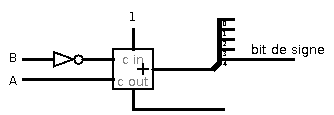
\includegraphics[width=6cm]{comparateur}

  \end{solution}
\end{enumerate}

\section{Quine-McCluskey}
\begin{enumerate}
  \item $f(a,b,c,d) = \Sigma m(4,5,6,7,12,13,14,15)$, on donne la colonne $2^2$
    de la table de QMC. Donner la colonne $2^3$ et retrouver ce résultat par la
    table de Karnaugh.

    \begin{center}
    \begin{tabular}{cll}
              & $2^2$ & $2^3$ \\
      \hline
      4,5,6,7     & \verb!01--!  &\\
      4,5,12,13   & \verb!-10-!  &\\
      4,6,12,14   & \verb!-1-0!  &\\
      \hline
      5,7,13,15   & \verb!-1-1!  &\\
      6,7,14,15   & \verb!-11-!  &\\
      12,13,14,15 & \verb!11--!  &\\
      \hline
    \end{tabular}
    \end{center}

    \begin{solution}
      On retrouve un seul implicant premier: \verb!-1--!.
      L'implicant est donc essentiel et $f=b$
      Sur le tableau de Karnaugh on peut ainsi regrouper tous les 1
      dans un rectangle de taille 8.
    \end{solution}

    \item Donner tous les implicants de la fonction $f(a,b,c) = \Sigma
      m(0,1,5,7)$

      \begin{solution}
        \begin{center}
          \begin{tabular}{cll}
            $2^0$& $2^1$& \\
            \hline
            \verb!0000!& \verb!000-!  &\\
            \hline
            \verb!0001!& \verb!0-01!  &\\
            \hline
            \verb!0101!& \verb!01-1!  &\\
            \hline
            \verb!0111!&  &\\
            \hline
          \end{tabular}
        \end{center}

        On trouve trois implicants. Les implicants 1 et 3 sont essentiels.
        \begin{tabular}{ccccc}
          &0&1&5&7\\
          \hline
       0,1&X&X& & \\
       1,5& &X&X& \\
       5,7& & &X&X\\
        \end{tabular}
      \end{solution}


    \item On considère la table des implicants ci-dessous.
      \begin{enumerate}
        \item Simplifiez la et déduisez en une forme disjonctive minimale.
          \begin{solution}
            On peut remarquer pour la simplification que $\overline{c}d$ est
            inclus dans $bd$.
          \end{solution}
        \item Donnez toutes les formes disjonctives minimales possibles.
          \begin{solution}
            \begin{itemize}
              \item $bd + \overline{a}b$
              \item $bd + b\overline{c}$
              \item $\overline{a}b + b\overline{c}$
              \item $\overline{a}b + \overline{c}d$
            \end{itemize}
          \end{solution}
      \end{enumerate}

      \begin{center}
      \begin{tabular}{c|c|c|c|c|}
                       & $m_4$& $m_5$ & $m_7$ & $m13$\\
                       \hline
        $b.d$           &   & X & X & X \\
        $b.\overline{c}$& X & X &   & X \\
        $\overline{a}.b$& X & X & X &   \\
        $\overline{c}.d$&   & X &   & X
      \end{tabular}
      \end{center}
    \item Mêmes questions pour la table des implicants ci-dessous.
      \begin{center}
      \begin{tabular}{c|c|c|c|c|c|c|c|c|c|c|}
                                   &0&1&2&5&6&7&8&9&10&14\\
                                   \hline
        $\overline{b}.\overline{c}$ &X&X& & & & &X&X&  &  \\
        $\overline{b}.\overline{d}$ &X& &X& & & &X& &X &  \\
        $c.\overline{d}$            & & &X& &X& & & &X &X \\
        $\overline{a}.\overline{c}.d$& &X& &X& & & & &  &  \\
        $\overline{a}.b.d$           & & & &X& &X& & &  &  \\
        $\overline{a}.b.c$           & & & & &X&X& & &  &
      \end{tabular}
      \end{center}

      \begin{solution}
        $\overline{b}.\overline{c} + \overline{c}.d + \overline{a}.b.d$
      \end{solution}

    \item $f(a,b,c,d)=\Sigma m(4,8,10,11,12,15) + d(9,14)$:
      \begin{enumerate}
        \item Déterminer les nombres binaires correspondant aux décimaux et les
          répartir en groupes (en fonction du nombre de bits à 1).
        \item Déterminer les implicants premiers de la fonction.
        \item Construire la table des implicants et déterminer les implicants
          premiers essentiels.
        \item Déterminer une solution minimale.
        \item Déterminer toutes les solutions minimales.
      \end{enumerate}

      \begin{solution}
        (La table ci-dessous a été générée avec l'excellent logiciel libre
        Bmin de J. Zelenka)

        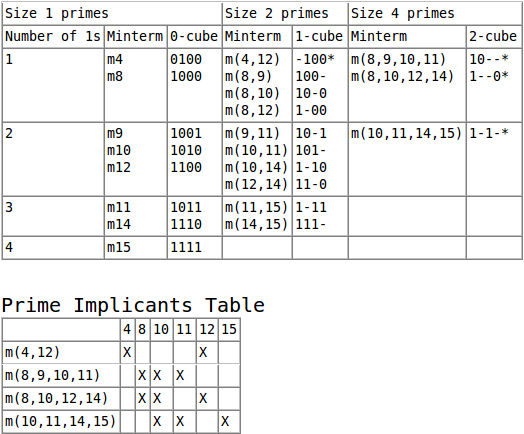
\includegraphics[width=8cm]{QMC1}

        Le premier et dernier implicants sont essentiels. On aboutit à deux
        expressions minimales possibles:
        \begin{itemize}
          \item $b.\overline{c}.\overline{d} + a\overline{d} + a.c$
          \item $b.\overline{c}.d + a\overline{b} + a.c$
        \end{itemize}
      \end{solution}

    \item Simplifier avec la méthode de QMC l'expression $f(a,b,c,d,e)=\Sigma
      m(0,2,3,5,7,9,11,13,14,16,18,24,26,28,30)$.
      \begin{solution}

        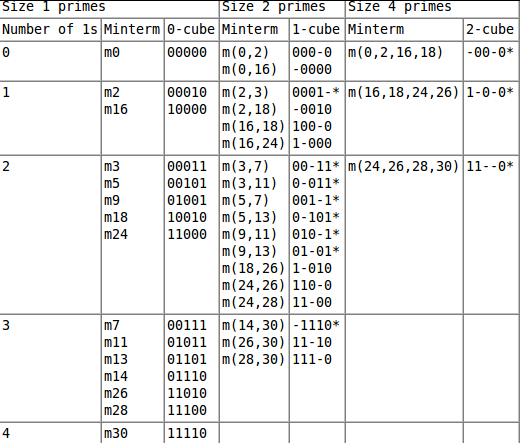
\includegraphics[width=8cm]{QMC2a}

        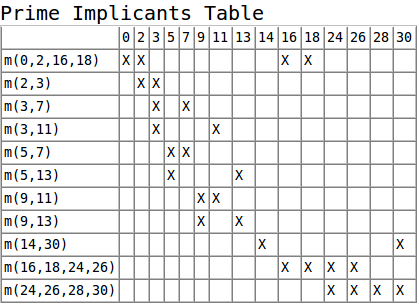
\includegraphics[width=6cm]{QMC2b}


        Une solution minimale est: $\overline{E}.\overline{C}.\overline{B} +
        \overline{E}.D.C.B + \overline{E}.B.A + E.D.\overline{B}.\overline{A} +
        E.\overline{D}.\overline{C}.\overline{A} + E.\overline{C}.B.\overline{A}$.
      \end{solution}
\end{enumerate}

\section{Circuit Multiplieur}

On souhaite réaliser un circuit multiplieur.
\begin{enumerate}
  \item Réaliser à la main la multiplication de $1011 \times 1100$.
  \item Construire un circuit qui multiplie deux nombres positifs
    sur 4 bits. Vous disposez d'additioneurs 4 bits.
    \begin{solution}
      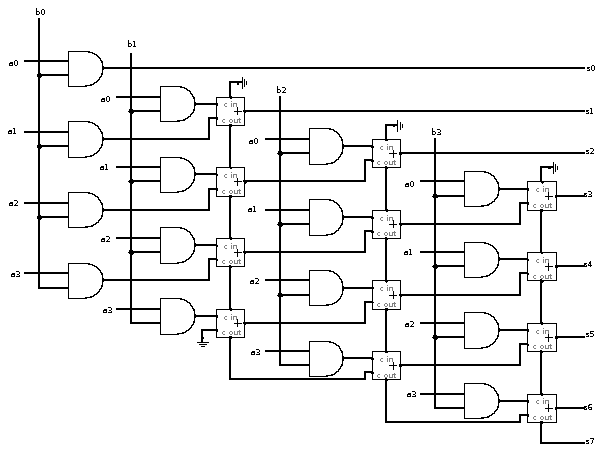
\includegraphics[width=10cm]{4-mult}
    \end{solution}

  \item Ce schéma marche t'il pour des entrées codées en complément à 2.
    Si ce n'est pas le cas, comment faudrait-il le modifier ?
    \begin{solution}
      $$B \times A = ( -A \times b_3).2^3 + (A \times b_2).2^2 + (A \times
      b_1).2 + (A \times b_0)$$

      Il faut prendre en compte deux facteurs:
      \begin{itemize}
        \item Dans le dernier étage il faut utiliser $-A = \overline{A} + 1$.
        \item Dans tous les étages il faut penser à propager le bit de signe
          pour faire la somme des produits partiels.
      \end{itemize}

      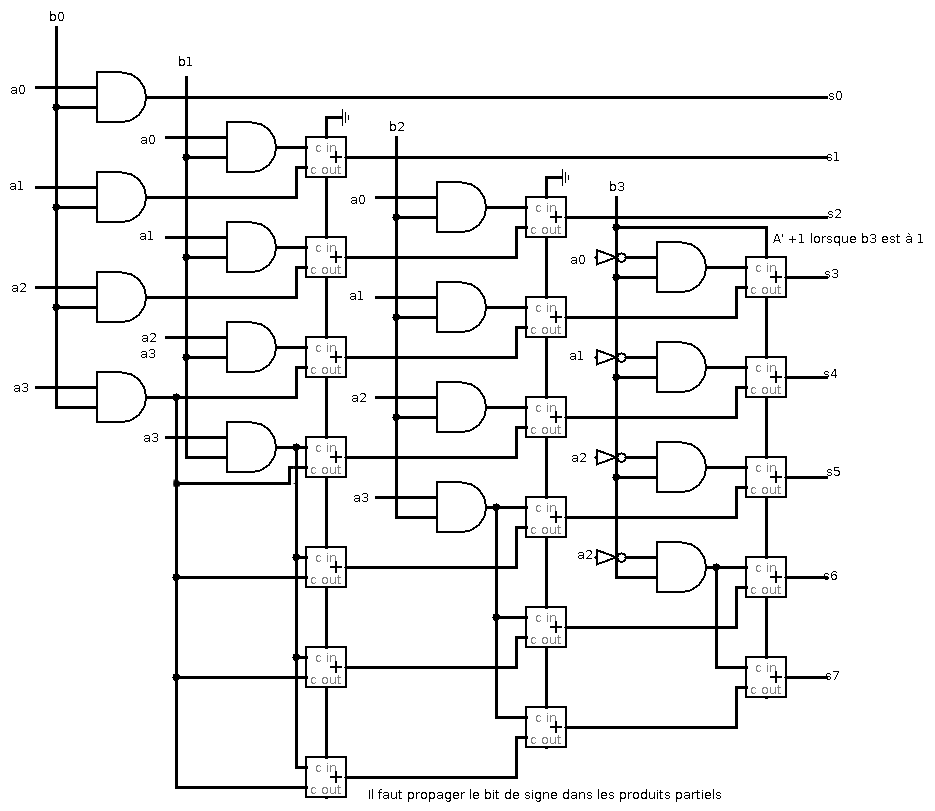
\includegraphics[width=10cm]{4-mult-CA-2}
    \end{solution}

\end{enumerate}

\end{document}
